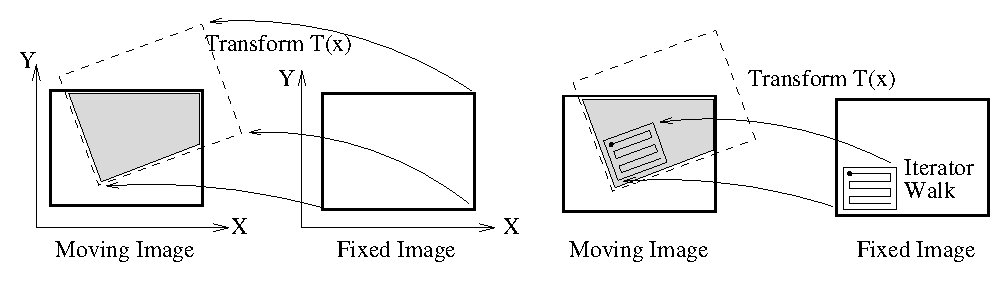
\includegraphics{ImageOverlap.eps}

An Image A is mapped over an image B by using a Transform


\subsection{Iterator Walking over a Region}

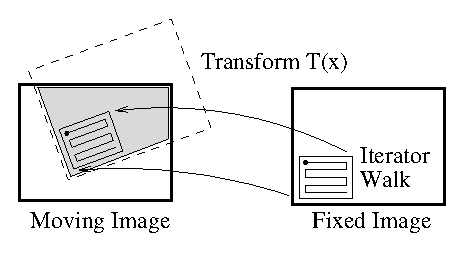
\includegraphics{ImageOverlapIterator.eps} 

An Iterator walking over a region of
B gets mapped on top of a blue region of A

\subsection{Need for an Interpolator}

The positions of the iterator are mapped
on non-grid positions in the image A 

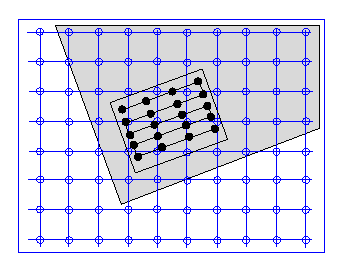
\includegraphics{ImageOverlapInterpolator.eps}

An interpolation is needed for estimating
the value of the image A at these non-grid positions.


\subsection{Overlaped regions }

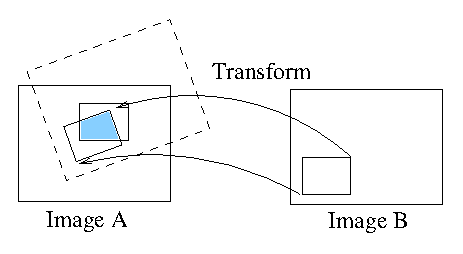
\includegraphics{ImageOverlapedRegions.eps}

Image metrics perform the computation over the intersection of a region in
image A and the map of a region in image B.


